\usetikzlibrary{patterns}


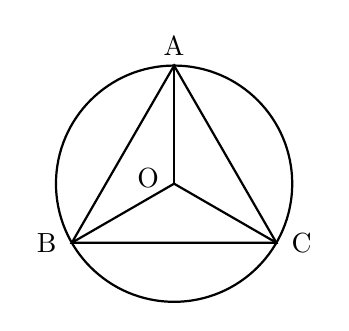
\begin{tikzpicture}[scale=1]

    % Define the center of the circle
    \coordinate (O) at (0,0);

    % Draw the outer circle
    \draw[thick] (O) circle (1.5);

    % Define the vertices of the inscribed triangle on the circle
    % A is positioned at the top (90 degrees)
    \coordinate (A) at (90:1.5);
    % B is positioned at the bottom-left (210 degrees)
    \coordinate (B) at (210:1.5);
    % C is positioned at the bottom-right (330 degrees)
    \coordinate (C) at (330:1.5);

    % Draw the edges of the inscribed triangle ABC
    \draw[thick] (A) -- (B) -- (C) -- cycle;

    % Draw the line segments from the center O to each vertex
    \draw[thick] (O) -- (A);
    \draw[thick] (O) -- (B);
    \draw[thick] (O) -- (C);

    % Place the labels for the vertices and the center point
    \node[above] at (A) {A};
    \node[left, xshift=-2pt] at (B) {B};
    \node[right, xshift=2pt] at (C) {C};
    % Place the label O slightly to the left of the center as shown in the image
    \node[left, xshift=-2pt, yshift=2pt] at (O) {O};

\end{tikzpicture}